\documentclass{article}

\usepackage{lipsum}
\usepackage{geometry}
\usepackage{hyperref}
\usepackage{xcolor}
\usepackage{graphicx}
\usepackage{listings}
\usepackage[framemethod=tikz]{mdframed}
\usepackage{bold-extra}

% links
\hypersetup{
  colorlinks=true,
  linkcolor=red,
  urlcolor=blue
}



% abbreviations
\newcommand{\eg}{\emph{e.g.}}
\newcommand{\ie}{\emph{i.e.}}
\newcommand{\cfr}{\emph{cfr.}}
\newcommand{\etc}{\emph{etc.}}



% custom colors
\definecolor{mygreen}{rgb}{0, 0.6, 0}
\definecolor{myllgray}{rgb}{0.95, 0.95, 0.95}
\definecolor{myddgray}{rgb}{0.25, 0.25, 0.25}
\definecolor{myblue}{rgb}{0, 0.3, 0.8}


% environment for C++ code
\lstdefinestyle{mycpp}{
  basicstyle=\small\ttfamily,
  %frame=single,
  language=C++,
  %backgroundcolor=\color{myllgray},
  commentstyle=\color{mygreen},
  keywordstyle=\color{myblue},
  numbers=left,
  numbersep=5pt,
  numberstyle=\footnotesize\color{black},
  %stringstyle=\color{orange},
  showstringspaces=false,
  xleftmargin=.05\textwidth,
}



% environment for bash/terminal code
\lstdefinestyle{myterm}{
basicstyle=\small\ttfamily,
%language=bash,
commentstyle=\color{mygreen},
keywordstyle=\bfseries,
numbers=none,
showstringspaces=false,
xleftmargin=.5\parindent,
}



% environment for CMake code
\lstdefinestyle{mycmake}{
  basicstyle=\small\ttfamily,
  %frame=single,
  %backgroundcolor=\color{myllgray},
  commentstyle=\color{mygreen},
  morecomment=[l][\color{mygreen}]{\#},
  numbers=left,
  numbersep=5pt,
  numberstyle=\footnotesize\color{black},
  showstringspaces=false,
  keywords=[1]{
    cmake_minimum_required,
    project,
    add_executable,
    add_library,
    add_subdirectory,
    target_include_directories,
    target_link_libraries,
    set,
  },
  keywordstyle=[1]\color{myblue},
  keywords=[2]{
    VERSION,
    PUBLIC,
    PROJECT_NAME,
    CMAKE_CXX_STANDARD,
  },
  keywordstyle=[2]\color{red},
}

\title{PROAV - Four in a Row in C++}
\date{}




\begin{document}
  
\maketitle


This Lab consists in programming the popular game \href{https://en.wikipedia.org/wiki/Connect_Four}{Four in a Row} in C++, in a simple graphical environment. The library that will be used for this purpose is called \href{https://bernhardfritz.github.io/piksel/}{piksel}, whose code is freely available in a \href{https://github.com/bernhardfritz/piksel}{github repository}.

\begin{figure}[htbp]
  \centering
  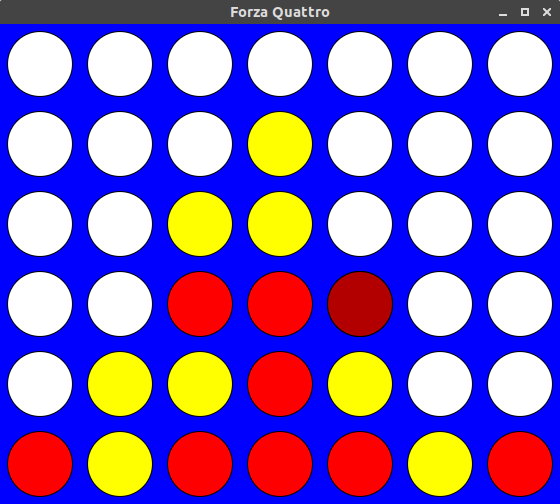
\includegraphics[width=.55\textwidth]{f4}
  \caption{The Four in a Row game created using piksel.}
\end{figure}

\section{Using piksel}

To make sure that you will be able to do the lab, we will first download and test the piksel library. Afterwards, you will be given information about few useful methods that you will need to create the four in a row application.

\subsection{Compiling the library}

Using a terminal, move to the main folder of the assignment and download piksel using:

\begin{center}
\ttfamily
git clone --recursive https://github.com/bernhardfritz/piksel.git
\end{center}

To test if everything works fine, create in the project root a new folder named \texttt{src}. Add the new file \texttt{piksel\_example.cpp} and paste the following code inside it\footnote{The file can be copied directly from \texttt{solution/src/piksel\_example.cpp}}:


\lstinputlisting[style=mycpp]{../solution/src/piksel_example.cpp}

To compile the code, add a \texttt{CMakeLists.txt} file inside the project root directory, and include the following lines of code\footnote{The name of the project corresponds to the Italian version of the game, feel free to name it differently.}:

\begin{lstlisting}[style=mycmake]
cmake_minimum_required(VERSION 3.1)
project(forza_quattro)

# use C++11 features
set(CMAKE_CXX_STANDARD 11)

# tell CMake to compile piksel as well
add_subdirectory(piksel)

# compile the example
add_executable(piksel_example src/piksel_example.cpp)
target_include_directories(piksel_example PUBLIC piksel/src)
target_link_libraries(piksel_example piksel)
\end{lstlisting}

Do not bother understanding it for now, we will come back to it in the next section. Time to compile: create a new folder named \texttt{build} and move inside it, then type the command \texttt{cmake~..} to start configuring. You might get an error concerning the version of CMake (piksel requires 3.12), but do not worry! The \href{https://bernhardfritz.github.io/piksel/#/gettingstarted/troubleshooting}{official solution} is to install the correct version of CMake, which does not require a lot of work. For simplicity, the steps are reported here:

\begin{center}
\begin{minipage}{.9\textwidth}
\begin{lstlisting}[style=myterm]
mkdir -p ~/programs_sources && cd ~/programs_sources
version=3.12
build=1
wget https://cmake.org/files/v$version/cmake-$version.$build.tar.gz
tar -xzvf cmake-$version.$build.tar.gz
cd cmake-$version.$build/
./bootstrap
make -j4
sudo make install
\end{lstlisting}
\end{minipage}
\end{center}

To check if the installation went fine, try to type \texttt{cmake --version} on your console: you should see the newly installed version 3.12.1. Also, as a good rule, do not delete the folder that contains the compiled CMake sources, \eg, \texttt{\textasciitilde/program\_sources/cmake\_3.12.1}. In fact, if in the future you wish to remove the installed version, it will suffice to move inside such directory and type \texttt{sudo make uninstall}. As a plus, from now on you can use the folder \texttt{program\_sources} to install programs from their sources.

\begin{mdframed}[hidealllines=true,backgroundcolor=red!20]
  \underline{\textsc{Be careful}}: by default, the new CMake will be installed in \texttt{/usr/local}. If you have already a CMake binary installed there, the procedures above might override it completely. For a safer procedure, make a backup before typing \texttt{sudo make install}. You can do that simply by running:
  \begin{center}
    \ttfamily
    sudo cp -p /usr/local/bin/cmake.3.10.1
  \end{center}
  The example assumes you have CMake 3.10.1 installed, change it to reflect the correct version!
\end{mdframed}

A ``quick-n-dirty'' workaround is also possible: simply open the file \texttt{piksel/CMakeLists.txt} and change the required version of CMake to the one that you have, \eg, 3.1. Note that with this solution the build might fail completely or that some piksel's functionalities might not work as intended.

Coming back to compiling piksel, after a successful configuration type \texttt{make} to build the executable and finally \texttt{./piksel\_example} to run it. You should see a rectangular window appearing in your screen, with a solid colored background. In addition, when moving the mouse inside the window, a white circle should be drawn following you. If so, then congratulations, piksel has been correctly compiled!




\subsection{Understanding piksel's fundamental classes}

Applications in piksel are rather simple: they all inherit from the base class \texttt{BaseApp}, which exposes a couple of virtual methods that can be overridden to customize the behavior of the program. In particular, the methods we are interested in are:

\begin{description}
  \item[\ttfamily BaseApp(int,int,std::string)] Constructor, takes the size (in pixels) of the window and optionally a string representing the ``title'' of the application.
  \item[\ttfamily virtual void setup()] Called once as soon as the application starts.
  \item[\ttfamily virtual void draw(piksel::Graphics\&)] Called repeatedly by the application, each call can be used to ``render'' a single frame. The \texttt{Graphics} object can be used to add shapes inside the window.
  \item[\ttfamily virtual void mousePressed(int)] Called when a mouse button is pushed down (not ``clicked''). The integer parameter allows to distinguish between different buttons on the mouse.
  \item[\ttfamily virtual void mouseMoved(int,int)] Executed when the mouse changes position inside the window. The two input variables correspond to the current horizontal and vertical coordinates (in pixels) of the device.
  \item[void run()] This is the ``entry-point'' of the application (generally invoked in \texttt{main}). You can think of it as a call to \texttt{setup} followed by an infinite loop that repeatedly calls \texttt{draw}.
\end{description}

The other fundamental class used in this library is \texttt{Graphics}, which is used to draw inside the canvas. We will not go into details, and we will just focus on few methods:

\begin{description}
  \item[void background(glm::vec4)] Allows to set the color of the background to the given one.
  \item[void ellipse(float,float,float,float)] Draws an ellipse in the specified coordinates (first two parameters of the function) with given width and height (third and fourth variables).
  \item[void fill(glm::vec4)] Changes the color used to draw shapes, such as ellipses.
  \item[void text(std::string,float,float)] Prints some text at the given coordinates.
  \item[void textSize(float)] Changes the size for following calls to \texttt{text}.
\end{description}

Finally, colors are all declared using the class \texttt{glm::vec4}, whose constructor accepts four \texttt{float} parameters, representing the RGBa (red, green, blue and alpha) components of the color, all normalized between 0 and 1.

Looking at the example code compiled in the previous section, it should be rather easy to understand what happens. First of all, we create a new class \texttt{App}, inheriting from \texttt{BaseApp}. The constructor simply initializes the canvas by calling the constructor of the base class. \texttt{App} has three private members: the background color of the canvas and the ``recorded'' mouse position. The color is initialized to a random one in the \texttt{setup} method. We also override the virtual method \texttt{mouseMoved}, whose default implementation is empty, so that the new coordinates of the mouse are saved whenever it is moved. Finally, the \texttt{draw} method will fill the background with the random color generated in \texttt{setup} and also draw a circle of fixed size in the recorded mouse position. To actually run the code, in the \texttt{main} method we create an instance of \texttt{App} and ``execute'' it by calling \texttt{start} (inherited from \texttt{BaseApp}).

Hoping that everything is clear up to this point, we are ready to start the actual assignment!



\section{Four in a Row}

Let's start by introducing the rules of the game:
\begin{itemize}
  \item A rectangular grid of $R\times C$ cells is initially empty
  \item Each of the two players is assigned a color, either red or yellow
  \item Players alternate in selecting one column out of the $C$ available ones and they are not allowed to pass
  \item A fully filled column cannot be selected
  \item Once a column is selected, a chip is inserted in it reaching the lowest free cell
  \item The first player who aligns four or more chips in any direction (horizontal, vertical, diagonal) wins the game
\end{itemize}

With these rules in mind, it is decided to implement the game as follows:

\begin{itemize}
  \item An \emph{abstract} class \texttt{Player} provides the \emph{interface} for a player. It will expose a \emph{pure virtual method} called \texttt{choose} that asks to select a column. Concrete implementations of this class will define different strategies, \eg, using the mouse to select a column (human player) or randomly selecting a valid column (a very bad AI).
  \item The class \texttt{Board} will serve two objectives at the same time: on one hand, it will store and handle the grid by exposing methods to query/update cells content, and on the other hand it will take care of graphics management by inheriting from \texttt{BaseApp} and overriding some of its methods. 
\end{itemize}

\end{document}